\documentclass{standalone}
\usepackage{tikz}
\usetikzlibrary{shapes.geometric, arrows}

\tikzstyle{startstop} = [rectangle, rounded corners, minimum width=3cm, minimum height=1cm, text centered, draw=black, fill=red!30]
\tikzstyle{process} = [rectangle, minimum width=3cm, minimum height=1cm, text centered, draw=black, fill=orange!30]
\tikzstyle{arrow} = [thick,->,>=stealth]

\begin{document}

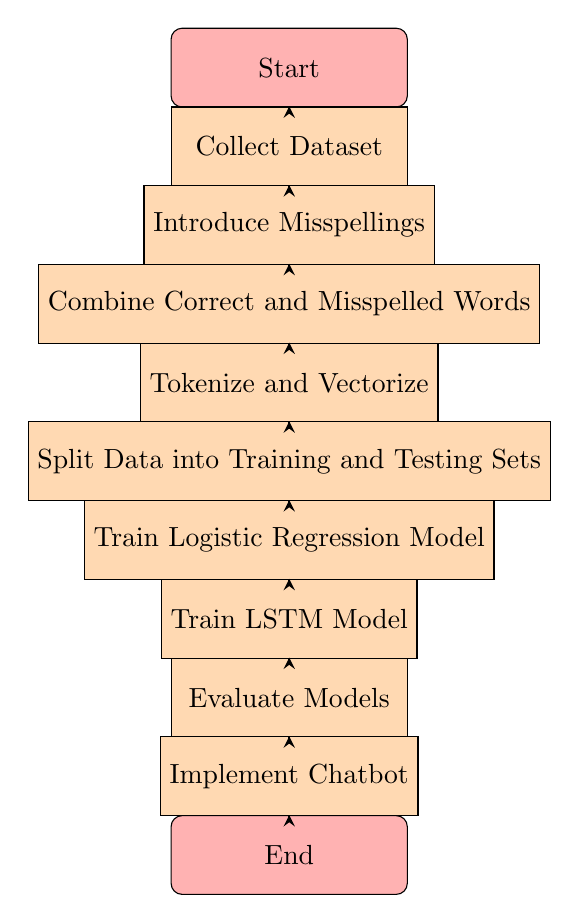
\begin{tikzpicture}[node distance=1cm]

\node (start) [startstop] {Start};
\node (collect) [process, below of=start] {Collect Dataset};
\node (introduce) [process, below of=collect] {Introduce Misspellings};
\node (combine) [process, below of=introduce] {Combine Correct and Misspelled Words};
\node (tokenize) [process, below of=combine] {Tokenize and Vectorize};
\node (split) [process, below of=tokenize] {Split Data into Training and Testing Sets};
\node (logreg) [process, below of=split] {Train Logistic Regression Model};
\node (lstm) [process, below of=logreg] {Train LSTM Model};
\node (evaluate) [process, below of=lstm] {Evaluate Models};
\node (chatbot) [process, below of=evaluate] {Implement Chatbot};
\node (end) [startstop, below of=chatbot] {End};

\draw [arrow] (start) -- (collect);
\draw [arrow] (collect) -- (introduce);
\draw [arrow] (introduce) -- (combine);
\draw [arrow] (combine) -- (tokenize);
\draw [arrow] (tokenize) -- (split);
\draw [arrow] (split) -- (logreg);
\draw [arrow] (logreg) -- (lstm);
\draw [arrow] (lstm) -- (evaluate);
\draw [arrow] (evaluate) -- (chatbot);
\draw [arrow] (chatbot) -- (end);

\end{tikzpicture}

\end{document}
